\documentclass[solution,letterpaper]{cs20}
\usepackage{enumerate}
\usepackage{tikz}
\usepackage{tikzit}
\usepackage{pgf}
\usepackage{hyperref}
\usepackage{qtree}
\usepackage{circuitikz}
\usepackage{amsmath}
\usepackage{float}
\usetikzlibrary{trees,positioning} \usetikzlibrary{arrows,automata} \usepackage{qtree} \input{tikzit.tikzstyles} \usetikzlibrary{trees,positioning} \usetikzlibrary{arrows,automata} \usepackage{qtree} \usetikzlibrary{arrows, automata} \usetikzlibrary{arrows, automata} \usetikzlibrary{trees,positioning} \usetikzlibrary{arrows, automata}
\begin{document}

    \header{6}{Simple Graphs Trees Rooted Trees Directed Graphs Properties of Relations Structural Induction  States and Invariants}


    \begin{problem}
        An CS20-incremental graph is built up in the following way.
        Start with a graph with a single vertex and no edges.
        The graph is incremented by repeatedly doing one of the
        following two steps:  either add a new vertex that is not
        adjacent to any existing vertices, or add a new vertex that is
        adjacent to all of the existing vertices.

        Prove by induction that if $G$ is a CS20-incremental graph, you can assign
        each vertex $u$ a rational number $x_u$ with $0 < x_u < 1$ such that
        any two vertices $v,w$ are adjacent in $G$ if and only if $
        x_v+x_w \geq 1$.
        (Note: these numbers do not have to be assigned when creating $G$,
        just there is a way to assign the numbers to a given incremental graph $G$.)

        \begin{solution}
            let us prove that for a CS20-incremental graph \( G \), we can assign each vertex \( u \) a rational number \( x_u \) such that \( 0 < x_u < 1 \) and any two vertices \( v \) and \( w \) are adjacent in \( G \) if and only if \( x_v + x_w \geq 1 \), through mathematical induction.

            In other words (by contra-positive), ($v$ and $w$ are adjacent $\to x_v + x_w \geq 1$ ) and ($v$ and $w$ are not adjacent $\leftarrow x_v + x_w < 1$ )


            \textbf{Base Case:}
            \( n = 1 \), the graph \( G \) has only one vertex and no edges. We can assign \( x_1 \) to be 0.5 such that if the one node in $G$ is considered adjacent to itself, $x_1 + x_1 \geq 1$ or $0.5 + 0.5 \geq 1.$

            \textbf{Inductive hypothesis:}
            Assume the statement is true for all CS20-incremental graphs with \( n \) vertices. We will prove it for a graph \( G \) with \( n+1 \) vertices.

            \textbf{Inductive step:}
            Let \( G \) be a CS20-incremental graph with \( n+1 \) vertices. We will consider two cases for how \( G \) could be constructed from a graph \( G' \) with \( n \) vertices.

            \textbf{Case 1: Adding a vertex that is not adjacent to any existing vertices}

            In this case, let \( G' \) be the CS20-incremental graph with \( n \) vertices, and \( v \) be the n+1-th vertex.
% In \( G' \), the vertices are each assigned rational numbers \( x_1, x_2, \ldots, x_n \) such that \( x_i + x_j \geq 1 \) if and only if vertices \( i \) and \( j \) are adjacent.

            In \( G \), the new vertex \( v \) is not adjacent to any vertex in \( G' \). To ensure that \( x_v + x_i < 1 \) for all \( i \) (where \( i \) denotes vertices in \( G' \)), choose \( x_v \) such that \(x_v \leq 1 - \text{min}(x)\) or more precisely if we consider $p, q \in \mathbb{Z}$ such that $\frac{p}{q} = \text{min}(x)$, let $x_v = \frac{p}{q + 1}$.

            Now, any two vertices \( i \) and \( j \) in \( G' \) will satisfy \( x_i + x_j \geq 1 \) if and only if they are adjacent, as assumed by the inductive hypothesis. For \( v \) and any vertex \( i \) in \( G' \), \( x_v + x_i < 1\) which holds even for even the edge cases such was when we must consider the largest vertex in $G$ (let $\frac{p}{q}$ = the largest vertex in $G$ where $p,q \in \mathbb{Z}$): because $1 - \frac{p}{q} + \frac{p}{q + 1} \leq 1$ , which is consistent with the fact that \( v \) is not adjacent to any vertex in \( G' \).
            Therefore, the assignment \( x_v = \frac{p}{q+1} \) satisfies the conditions that ($v$ and $w$ are adjacent $\to x_v + x_w \geq 1$ ) and ($v$ and $w$ are not adjacent $\leftarrow x_v + x_w < 1$ )

            \textbf{Case 2: Adding a vertex that is adjacent to all existing vertices}

            In this case, let \( G' \) be the CS20-incremental graph with \( n \) vertices, and \( v \) be the \( n+1 \)-th vertex added. The new vertex \( v \) is adjacent to all vertices in \( G' \). Let the vertices in \( G' \) have rational numbers \( x_1, x_2, \ldots, x_n \) such that \( x_i + x_j \geq 1 \) if and only if vertices \( i \) and \( j \) are adjacent.

            Let us assign $v$ a rational value $x_v = \frac{p+1}{q+1}$ where $p,q \in \mathbb{Z}$ and $\frac{p}{q} = 1 - \text{min}(x)$. Since $\frac{p+1}{q+1} > \frac{p}{q}$, the sum of any two vertices (which must be adjacent) therefore will be $1 - \frac{p}{q} + \frac{p+1}{q+1} \geq 1$. As a result the condition  ($v$ and $w$ are adjacent $\to x_v + x_w \geq 1$ ) and ($v$ and $w$ are not adjacent $\leftarrow x_v + x_w < 1$ ) hold true.\\
            \textbf{Conclusion:} \\
            For any CS20-incremental graph \( G \) with \( n \) vertices, it is possible to assign each vertex a rational number \( x_u \) such that \( 0 < x_u < 1 \) and any two vertices \( v \) and \( w \) are adjacent in \( G \) if and only if \( x_v + x_w \geq 1 \).
        \end{solution}
    \end{problem}
    \newpage

    \begin{problem}
        \begin{itemize}
            \item Let $A,B$ be two subsets of $\{1,2,\ldots,n\}$ with $|A| > n/2$ and $|B| > n/2$.
            Prove that $A \cap B$ is nonempty.
            \item Let $G$ be an undirected graph on $n$ vertices, where each vertex has degree at
            least $n/2$.  Prove that $G$ is connected.
        \end{itemize}

        \begin{solution}
        (1) \\
        Let us prove that for two subsets $A,B$ of $\{1,2,\ldots,n\}$ with $|A| > n/2$ and $|B| > n/2$, $A \cap B$ is nonempty by contradiction. \\
        Assume $A \cap B$ is empty.  \\
        Consider the cardinality of $A \cup B$. Since $A \text{ and } B \text{ are disjoint, we have}$ \\
        $|A \cup B| = |A| + |B|$ \\
        $\text{Given that } |A| > \frac{n}{2} \text{ and } |B| > \frac{n}{2}, \\
        |A| + |B| > \frac{n}{2} + \frac{n}{2} \\
        |A| + |B| > n \\
        \text{Unfortunately, the set } \{1, 2, \ldots, n\} \text{ has only } n \text{ elements } \\
        \text{and} A \cup B \text{ cannot have more than } n \text{ elements. This contradiction means that our assumption is false.} \\
        \text{Therefore, } A \cap B \text{ must be nonempty.}$ \\

        (2) \\
        Let us prove that for an undirected graph $G$ with n vertices, where each vertex has a degree at least n/2, that G is connected by contradiction. \\
        Assume for contradiction that $G$ is not connected. Then $G$ can be partitioned into at least two non-empty disjoint subgraphs $G_1$ and $G_2$ such that there are no edges between $G_1$ and $G_2$. \\

        Let $|G_1| = k$ and $|G_2| = n - k$ therefore $ 1 \leq k \leq n-1.$ \\

        Every vertex in $ G_1 $ has a degree of at least $ \frac{n}{2}$.  Therefore, each vertex in $ G_1 $ is connected to at least $ \frac{n}{2} $ vertices. The maximum number of vertices a vertex in $ G_1 $ can be connected to within $ G_1 $ is $ k-1$. \\

        Since each vertex in $ G_1 $ has a degree of at least $ \frac{n}{2}$, we must have $k-1 \geq \frac{n}{2}$.
        Similarly, for $G_2$, each vertex must be connected to at least $ \frac{n}{2}$ vertices, and the maximum number of vertices within $ G_2 $ is $ n-k-1. $ Therefore, we have

        $n-k-1 \geq \frac{n}{2}$.

        From $ k-1 \geq \frac{n}{2}$, we get $ k \geq \frac{n}{2} + 1$.

        From $ n-k-1 \geq \frac{n}{2}$,  we get $ n-k \geq \frac{n}{2} + 1$, which implies $ k \leq \frac{n}{2} - 1$

        These two inequalities $ k \geq \frac{n}{2} + 1 $ and $ k \leq \frac{n}{2} - 1 $ are contradictory. Therefore, our initial assumption that $ G $ is not connected must be false.
        Therefore, $G$ must be connected.
        \end{solution}
    \end{problem}
    \newpage

    \begin{problem}
        Let $G$ be a graph with $n$ vertices and $m$ edges. Prove by induction that $G$ has at least
        $m- n + 1$ cycles.  (You may use the fact that a graph with $n$ vertices and $n$ or more edges
        has a cycle.)

        \begin{solution}

            Let \( G \) be a graph with \( n \) vertices and \( m \) edges. We want to prove that \( G \) has at least \( m - n + 1 \) cycles.\\
            \textbf{Base Case} \\
            Consider the case where \( m = n - 1 \).
            A graph with \( n \) vertices and \( n - 1 \) edges is a tree (since a tree with \( n \) vertices has exactly \( n - 1 \) edges and no cycles). A tree has 0 cycles.
            For \( m = n - 1 \): $m - n + 1 = (n - 1) - n + 1 = 0$
            Thus, the number of cycles in a tree matches our claim for this base case.

            \textbf{Inductive Step} \\
            Assume the statement is true for a graph with \( n \) vertices and \( k \) edges, where \( k \geq n - 1 \). Specifically, assume such a graph has at least \( k - n + 1 \) cycles.
            We need to show that the statement holds for a graph with \( n \) vertices and \( k + 1 \) edges.
            Consider a graph \( G' \) with \( n \) vertices and \( k + 1 \) edges. Let \( e \) be an edge in \( G' \). Remove the edge \( e \) from \( G' \) to obtain a graph \( G \) with \( n \) vertices and \( k \) edges.

            By the inductive hypothesis, the graph \( G \) with \( n \) vertices and \( k \) edges has at least \( k - n + 1 \) cycles. \\ When the edge \( e \) is added back to \( G \) to form \( G' \), it either: \\

            1) Creates a cycle, in which case the number of cycles in \( G' \) increases by 1, or \\
            2) Connects two previously disconnected components, forming exactly one new cycle. \\

            In either case, adding \( e \) results in exactly one additional cycle. Therefore, the number of cycles in \( G' \) is at least \( (k - n + 1) + 1 = k - n + 2 \).

            For \( G' \) with \( k + 1 \) edges, the number of cycles should be at least: $(k + 1) - n + 1 = k - n + 2$
            Therefore, the inductive step holds true.

            \textbf{Conclusion}

            By mathematical induction, the statement holds for all graphs with \( n \) vertices and \( m \) edges. Therefore, any graph with \( n \) vertices and \( m \) edges has at least \( m - n + 1 \) cycles.

        \end{solution}
    \end{problem}
    \newpage

    \begin{problem}
        Consider a rooted tree that has a special vertex (the root), and
        directed edges.  The root vertex is connected to $d$ additional nodes,
        which are called its children; the edges point up from the children to the
        root.  Each child of the root in turn has $d$ children, with those children directed
        up to the parent, and so on.  This is called a rooted $d$-ary tree.
        \begin{itemize}
            \item
            ind a formula for the number of total nodes of a rooted $d$-ary
            tree with $k$ levels.  (The root is level 0, the children of the root
            are level 1, etc. so $k$ levels means the tree ends at level $k-1$.)
            The formula should NOT be expressed as a sum of $\approx k$ terms;
            simplify the epxression.
            \item
            Rooted $d$-ary trees are a good model for chain letter pyramid scams.
            Explain how to determine how much would be expected to make in the
            following chain letter, from the 1930s.
        \end{itemize}

        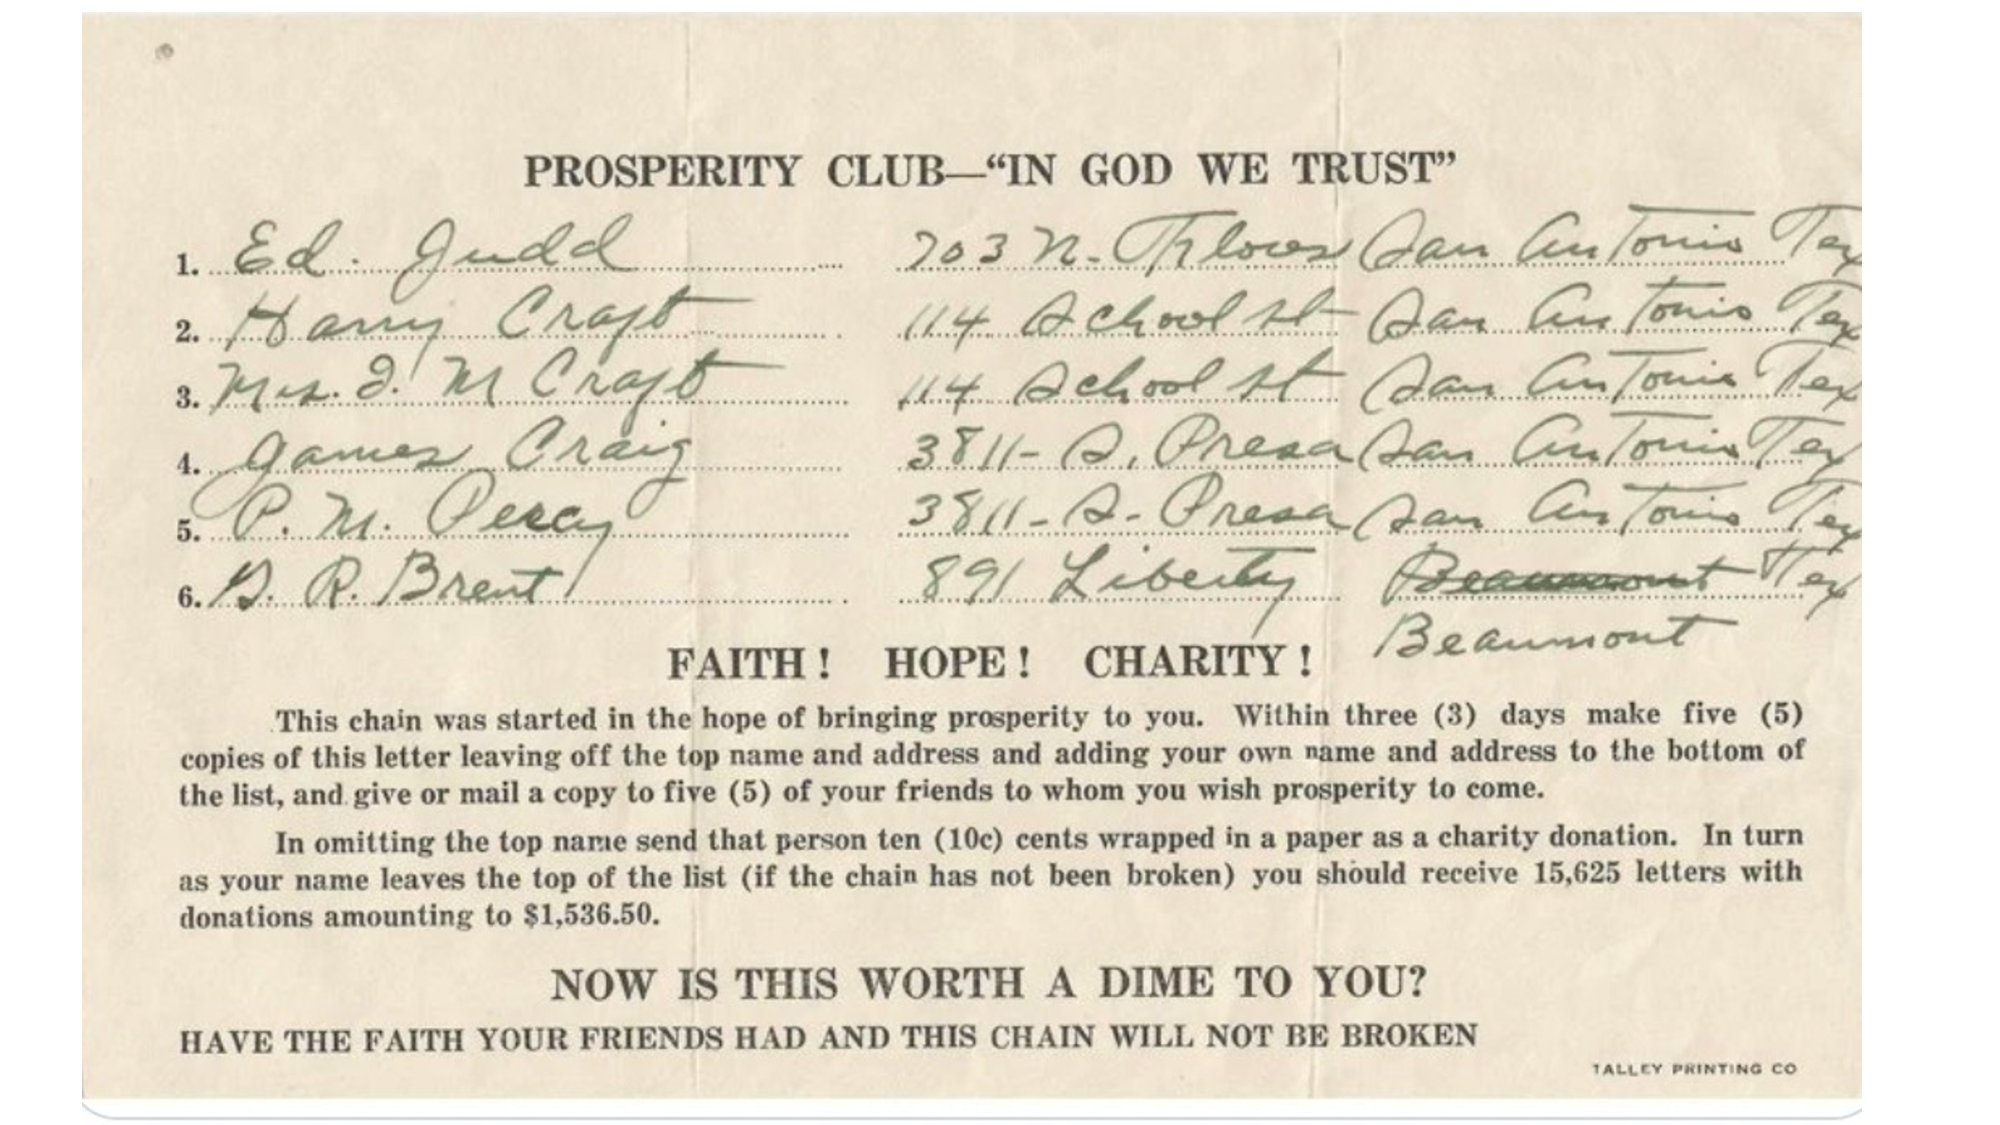
\includegraphics[width=10cm]{ChainMailLetter.pdf}

        \begin{solution}
            1) $\sum{d^i}^{k-1}_{i=0} = \frac{d^k - 1}{d - 1} \because \text{geometric sum}$ \\
            2) $0.1 * 5^6 = \$1,536.5$
        \end{solution}
    \end{problem}
    \newpage

    \begin{problem}

        Let $R$ and $S$ be equivalence relations on a set $X$.

        \subproblem Prove that $T=R \cap S$ is also an equivalence relation on $X$.
        \subproblem Is $V=R \cup S$ also an equivalence relation $X$?  Prove it if it is,
        or show a counterexample if it is not.

        \begin{solution}
        (A)\\
        To prove that \( T \) is an equivalence relation, we need to show that it satisfies the properties of reflexivity, symmetry, and transitivity. \\
        \textbf{Reflexivity}
        For \( T \) to be reflexive, we need to show that \(\forall x \in X, (x, x) \in T\). Since \( R \) and \( S \) are equivalence relations, they are reflexive. Therefore, \(\forall x \in X, (x, x) \in R\) and \((x, x) \in S\). By the definition of \( T = R \cap S \), \(\forall x \in X, (x, x) \in R \cap S\), which implies \((x, x) \in T\). therefore, \( T \) is reflexive.\\
        \textbf{Symmetry}
        For \( T \) to be symmetric, we need to show that \(\forall x, y \in X, (x, y) \in T \implies (y, x) \in T\). Suppose \((x, y) \in T\). This means \((x, y) \in R\) and \((x, y) \in S\). Since \( R \) and \( S \) are symmetric, \((x, y) \in R \implies (y, x) \in R\) and \((x, y) \in S \implies (y, x) \in S\). Therefore, \((y, x) \in R\) and \((y, x) \in S\), which implies \((y, x) \in R \cap S\), and hence \((y, x) \in T\). therefore, \( T \) is symmetric.\\
        \textbf{Transitivity}
        For \( T \) to be transitive, we need to show that \(\forall x, y, z \in X, (x, y) \in T \wedge (y, z) \in T \implies (x, z) \in T\). Suppose \((x, y) \in T\) and \((y, z) \in T\). Which means \((x, y) \in R\) and \((x, y) \in S\), and \((y, z) \in R\) and \((y, z) \in S\). Since \( R \) and \( S \) are transitive, \((x, y) \in R \wedge (y, z) \in R \implies (x, z) \in R\) and \((x, y) \in S \wedge (y, z) \in S \implies (x, z) \in S\). Therefore, \((x, z) \in R\) and \((x, z) \in S\), which implies \((x, z) \in R \cap S\), and hence \((x, z) \in T\). therefore, \( T \) is transitive. \\
        Since \( T \) satisfies reflexivity, symmetry, and transitivity, \( T = R \cap S \) is an equivalence relation on \( X \).

        (B) \\
        To determine whether \( V \) is an equivalence relation, we need to check if it satisfies reflexivity, symmetry, and transitivity. \\
        \textbf{Reflexivity} \\
        For \( V \) to be reflexive, we need to show that \(\forall x \in X, (x, x) \in V\). Since \( R \) and \( S \) are equivalence relations, they are reflexive. Therefore, \(\forall x \in X, (x, x) \in R\) and \((x, x) \in S\). By the definition of \( V = R \cup S \), \(\forall x \in X, (x, x) \in R \cup S\), which implies \((x, x) \in V\). therefore, \( V \) is reflexive. \\
        \textbf{Symmetry} \\
        For \( V \) to be symmetric, we need to show that \(\forall x, y \in X, (x, y) \in V \implies (y, x) \in V\). Suppose \((x, y) \in V\). This means \((x, y) \in R\) or \((x, y) \in S\). Since \( R \) and \( S \) are symmetric, \((x, y) \in R \implies (y, x) \in R\) and \((x, y) \in S \implies (y, x) \in S\). Therefore, \((y, x) \in R\) or \((y, x) \in S\), which implies \((y, x) \in R \cup S\), and hence \((y, x) \in V\). therefore, \( V \) is symmetric. \\
        \textbf{Transitivity} \\
        For \( V \) to be transitive, we need to show that \(\forall x, y, z \in X, (x, y) \in V \wedge (y, z) \in V \implies (x, z) \in V\). Suppose \((x, y) \in V\) and \((y, z) \in V\). This means \((x, y) \in R\) or \((x, y) \in S\), and \((y, z) \in R\) or \((y, z) \in S\). We have several cases to consider:
        1)\((x, y) \in R\) and \((y, z) \in R\): Since \( R \) is transitive, \((x, y) \in R \wedge (y, z) \in R \implies (x, z) \in R \subseteq V\).
        2) \((x, y) \in S\) and \((y, z) \in S\): Since \( S \) is transitive, \((x, y) \in S \wedge (y, z) \in S \implies (x, z) \in S \subseteq V\).
        3) \((x, y) \in R\) and \((y, z) \in S\): We cannot conclude \((x, z) \in V\) because \((x, z)\) does not necessarily belong to either \( R \) or \( S \).
        4) \((x, y) \in S\) and \((y, z) \in R\): Similarly, we cannot conclude \((x, z) \in V\).
        Since \( V \) fails to satisfy transitivity in cases 3 and 4, \( V = R \cup S \) is not necessarily an equivalence relation. \\
        \textbf{Counterexample} \\
        Let \( X = \{a, b, c\} \). Define two equivalence relations: \\
        \( R = \{(a, a), (b, b), (c, c), (a, b), (b, a)\} \) \\
        \( S = \{(a, a), (b, b), (c, c), (b, c), (c, b)\} \) \\
        Then: \( R \cup S = \{(a, a), (b, b), (c, c), (a, b), (b, a), (b, c), (c, b)\} \)  \\

        In \( R \cup S \):\\
        \( (a, b) \in V \quad \text{and} \quad (b, c) \in V, \quad \text{but} \quad (a, c) \notin V \) \\
        Therefore, \( V \) is not transitive, and therefore, \( V \) is not an equivalence relation.
        \end{solution}
    \end{problem}
    \newpage

    \begin{problem}

        Bulgarian solitaire is a game played by one player. The game starts with 6 coins distributed in 1-6 piles. Then the player repeats the following step:

        \begin{itemize}
            \item Remove one coin from each existing pile and form a new pile.
        \end{itemize}

        The order of the piles doesn’t matter, so the state can be described as a sequence of positive integers in non-increasing order adding up to 6. For example, the first two moves when a player begins with two piles of 3 coins are $(3,3) \to (2,2,2)$ and $(2,2,2) \to (3,1,1,1)$. On the next move, the last three piles disappear, creating piles of 4 and 2 coins.

        \subproblem Trace the sequence of moves starting from two initial piles of 3 until it repeats.
        \subproblem Draw as a directed graph the complete state space with six coins.
        \subproblem Show that if the stacks are of heights $n, n-1, \ldots 1$ for any arbitrary number of coins $n$, the next configuration is the same.

        \begin{solution}
        (A) \\
        $(3,3) \to (2,2,2) \to (1,1,1,3) \to (4,2) \to (3,1,2) \to (2,1,3) \to (1,2,3) \to \cdots \to (1,2,3)$ \\
        (B) \\
        \begin{figure}[h]
            \centering
            \includegraphics[width=0.1\linewidth, angle=90]{IMG_4079.JPG}
            \label{fig:enter-label}
        \end{figure} \\
        (C) \\
        If the stacks are the form where their heights are $n, n-1, \cdots, 1$ the piles were always remain in that same state because there will always be a new stack of size n created, and each existing stack will be decremented by 1. \\
        1) Each stack is decremented by 1 ie the stacks will have heights $n-1, n-2, \cdots, 0$, however since there cannot be a zero height stack the total stack count decreases by 1. $\{n-1, n-2, \cdots, 0\} \equiv \{n-1, n-2, \cdots, 1 \}$ \\
        2) We will create a new stack of size n from the coins removed from existing stacks. There will be n removed coins because there was originally n stacks, and we took 1 coin from each (therefore we have n spare coins to make a stack). \\
        $\{n\} \cup \{n-1, n-2, \cdots, 1\} = \{n, n-1, \cdots, 1\}$


        \end{solution}
    \end{problem}
    \newpage

    \begin{problem}
        A robot named Wall-E wanders around a two-dimensional grid. He starts out at $(0,0)$ and is allowed to take four different types of steps:
        \begin{enumerate}
            \item $(+2, -1)$
            \item $(-1, +2)$
            \item $(+1, +1)$
            \item $(-3, +0)$
        \end{enumerate}

        Thus, for example, Wall-E might walk as follows. The types of his steps are listed above the arrows:

        \[(0,0)\xrightarrow{1}(2,-1)\xrightarrow{3}(3,0)\xrightarrow{2}(2,2)\xrightarrow{4}(-1,2)\]

        Wall-E’s true love, the fashionable and high-powered robot, Eve, awaits at $(0,2)$

        \subproblem Let Wall-E's movements be modeled by a state machine $M = \{\Sigma, S,\delta, s_0, F\}$. $\Sigma$ is the set of four actions defined above. Recall that $\delta : (s_1, \sigma) \to s_2$, where $s_1,s_2 \in S$ and $\sigma \in \Sigma$. And since we'll define success as Wall-E getting to Eve, we'll say that $F = \{(0,2)\}$. Provide definitions for:
        \begin{enumerate}
            \item the state space $S$
            \item the transition relation $\delta : (s_1, \sigma) \to s_2$, where $s_1,s_2 \in S$ and $\sigma \in \Sigma$ (you may define this relation by parts/cases), and
            \item $s_0$
        \end{enumerate}

        \subproblem Sadly, you can see that Wall-E will never be able to reach Eve. But Wall-E doesn't believe it. What preserved invariant could you use to prove to Wall-E that he can never reach Eve at $(0,2)$? \emph{Hint:} The value $x-y$ is not invariant, but how does it change?

        \subproblem Prove to Wall-E that he cannot reach Eve using your preserved invariant and Floyd's invariant principle.

        \begin{solution}
        (A) \\
        1. The state space $S$, is the list of all possible states Wall-E can inhabit. \\
        $\{x \in \mathbb{Z}^2: \exists k_1, k_2, k_3, k_4 \in \mathbb{N}. x = (2k_1 - 1k_2 + 1k_3 -3k_4, -1k_1 + 2k_2 + 1k_3 + 0k_4) \}$ \\
        ie. All possible compositions for state transitions 1,2,3,4. \\
        2. $\delta ((x, y), \sigma) =  \begin{cases}
        (x+2, y-1), & \sigma = 1 \\
        (x-1, y+2) & \sigma = 2 \\
        (x+1, y+1) & \sigma = 3 \\
        (x-3, y) & \sigma = 4 \\
        \end{cases} $ \\
        3. The start state ie. Wall-E's starting coordinate (0,0) \\

        (B) \\
        \( \text{The invariant is that } x - y = 0 \pmod{3} \), where \( x \) and \( y \) are Wall-E's current coordinates.

        \textbf{Case 1:} $(+2, -1)$: \\
        \((x, y) \to (x+2, y-1)\). \\
        The change in \( x - y \) is \((x + 2) - (y - 1) = x - y + 3\). \\
        Therefore, \( (x - y) \pmod{3} \) remains unchanged since \( x - y + 3 \equiv x - y \pmod{3} \). \\
        \textbf{Case 2:} $(-1, +2)$: \\
        \((x, y) \to (x-1, y+2)\). \\
        The change in \( x - y \) is \((x - 1) - (y + 2) = x - y - 3\). \\
        Therefore, \( (x - y) \pmod{3} \) remains unchanged since \( x - y - 3 \equiv x - y \pmod{3} \). \\
        \textbf{Case 3:} $(+1, +1)$: \\
        \((x, y) \to (x+1, y+1)\). \\
        The change in \( x - y \) is \((x + 1) - (y + 1) = x - y\). \\
        Therefore, \( (x - y) \pmod{3} \) remains unchanged. \\
        \textbf{Case 4:} $(-3, +0)$: \\
        \((x, y) \to (x-3, y)\). \\
        The change in \( x - y \) is \((x - 3) - y = x - y - 3\). \\
        Therefore, \( (x - y) \pmod{3} \) remains unchanged since \( x - y - 3 \equiv x - y \pmod{3} \). \\


        (C) \\
        Wall-E starts at $(0, 0)$: \\
        let I be our invariant \\
        \( I = x - y = 0 - 0 = 0 \) therefore, \( I = 0 \pmod{3} \).
        Eve is at $(0, 2)$: \\
        \( I = x - y = 0 - 2 = -2 \) \\
        Therefore, \( I = -2 \equiv 1 \pmod{3} \).
        The invariant \( x - y \pmod{3} \) remains unchanged for all the allowed moves of Wall-E. Since Wall-E starts at a position where \( x - y \equiv 0 \pmod{3} \), he can only visit positions where \( x - y \equiv 0 \pmod{3} \). However, Eve's position $(0, 2)$ corresponds to \( x - y \equiv 1 \pmod{3} \)., Wall-E can never reach Eve's position because the invariant values do not match.


        \end{solution}
    \end{problem}


\end{document}
